\documentclass[11pt]{article}

\usepackage[margin=1in]{geometry}
\usepackage[T1]{fontenc}
\usepackage[utf8]{inputenc}
\usepackage{lmodern}
\usepackage{amsmath,amssymb}
\usepackage{booktabs}
\usepackage{array}
\usepackage{graphicx}
\usepackage{caption}
\usepackage{enumitem}
\usepackage[round,authoryear]{natbib}
\usepackage[hidelinks]{hyperref}
\usepackage{url}
\usepackage{adjustbox}
\usepackage[section]{placeins}

\captionsetup{font=small,labelfont=bf}
\setlength{\parskip}{0.35em}
\newcommand{\USD}{\$}
\newcommand{\tabin}[2][\small]{{#1\input{tables/#2}}}
\newcommand{\tabfit}[1]{\begin{adjustbox}{max width=\linewidth,center}\small\input{tables/#1}\end{adjustbox}}

\title{When the Market Is Closed: Session-Dependent Adverse Selection for Liquidity Providers in 24/7 Tokenized-Equity AMMs}
\author{Kamal\thanks{The author develops Uptick, a vault product that builds on the replay engine described here (Appendix~\ref{app:product}).}\\[2pt]\small Uptick}
\date{October 2026}

\begin{document}
\maketitle

\begin{abstract}
Tokenized equities on Robinhood Chain trade against a dollar stablecoin in Uniswap pools around the clock, while the listed shares trade 32.5 hours a week and the Chainlink feeds that price them follow a 24/5 schedule. We ask when liquidity providers (LPs) in these pools lose to informed flow and whether calendar-aware ranges or fees recover the loss. We replay 5,113,049 swaps on three Stock Token pools over 54 days with a finite-position engine that charges fees and markouts under one consistent counterfactual, reported as two bounds. A static $\pm2\%$ position earns 3.94 to 33.27 dollars of fees per dollar of one-hour markout on weekends and 1.03 to 1.35 in NYSE hours (pooled 13.64 [4.41, 28.22] and 1.16 [0.91, 1.49], week-block 90\% intervals). The weekend ratio exceeds the NYSE ratio in 22 of 23 pool-weeks. The ordering holds at five-minute and one-hour horizons but weakens when weekend swaps are marked to the next open, and NYSE hours cannot be separated from weeknights on NVDA or TSLA 0.30\%. Fifteen Uniswap v4 pools replicate the weekend result but not the NYSE ranking. A pre-specified hours-aware range strategy meets its bar at point estimates on 2 of 3 tokens when rebalances pay only the pool fee and fails when they pay pool impact; its margin over the best static range has intervals that include zero, and it cannot be distinguished from randomly reassigned session labels in 56 of 64 cells. A session fee schedule adds 0.00 APR points out of sample, which follows from a volume elasticity below one and not from the data, so the test is uninformative; an oracle-gap surcharge changes sign with the sample split and the volume response. A weekend perpetual-futures price reduces Monday-open absolute error by 3.7\% [$-$4.6, 12.2], against 69.3\% [64.0, 73.4] at Monday 13:00 UTC.
\end{abstract}

\section{Introduction}\label{sec:intro}

Tokenized equities now trade on public blockchains at every hour of the week. On Robinhood Chain, an Arbitrum Orbit chain with chain identifier 4663, Robinhood-issued Stock Tokens trade against the USDG stablecoin in Uniswap v3 and v4 pools around the clock. The listed shares they track trade in a regular session that covers 32.5 of the 168 hours in a week, and the Chainlink equity feeds deployed on the chain follow a 24/5 schedule: across the three feeds we study, there was no update on any Saturday or Sunday of our sample and none on the Labor Day holiday. An automated market maker (AMM) liquidity provider in these pools sells immediacy at a fixed fee to whoever arrives, at any hour, against a reference market that is open for about a fifth of the week.

Two bodies of work give opposite intuitions about when that LP loses. Loss-versus-rebalancing theory \citep{milionis2022lvr} prices adverse selection off the variance of an external reference price, and equity microstructure shows that per-hour variance is many times higher while the exchange is open than while it is closed \citep{french1986variances}. Together they predict that LP losses concentrate in exchange hours. Fee hooks deployed or proposed for Stock Token pools charge the most when the market is closed, on the view that the weekend reopening gap is the main LP risk. Which view describes these pools is an empirical question, and its answer decides how an LP product should set ranges, fees and pool choice.

We answer it with four data sets drawn from the chain and from reference venues: every swap on three Stock Token/USDG Uniswap v3 pools over 54 days (5,113,049 swaps and \USD1,791.3M of volume), every swap on 15 Uniswap v4 Stock Token pools over 15.95 days (374,678 swaps), 168 ticker-weekends of Hyperliquid equity perpetual prices matched to Nasdaq official opens and closes, and a 49-hour census of 3,183,184 v4 swaps across all pools on the chain (used in Appendix~\ref{app:hooks}). Our contributions are as follows.

\begin{enumerate}[leftmargin=*,itemsep=2pt]
\item \textbf{A session profile of LP adverse selection in a 24/7 AMM whose reference market closes, with intervals and accounting bounds.} For a static $\pm2\%$ position, fees per dollar of one-hour markout are 1.03 to 1.35 in NYSE hours, 1.30 to 3.90 on weeknights and 3.94 to 33.27 on weekends across three pools. The weekend advantage over NYSE hours is the one result that survives every variant we ran (two accounting bounds, week-block and day-block resampling, three pool weightings, 5-minute and 1-hour horizons). NYSE hours are not separable from weeknights on NVDA or TSLA 0.30\%, and fees do not fall below markout in NYSE hours on pooled data.
\item \textbf{Horizon and pool-mix dependence, reported.} At six hours and at the next open the weeknight, not the regular session, is the most toxic session for NVDA; a sample of 15 v4 pools replicates the weekend result in 6 of 7 tickers but ranks NYSE hours as most toxic in only 4 of 8.
\item \textbf{A test of hours-aware ranges that does not support a calendar rule.} The pre-specified claim is met at point estimates under fee-only rebalancing costs and not under pool-impact costs; margins over the best static range carry intervals that include zero, and shuffled labels match the real calendar in most cells.
\item \textbf{A fee-schedule test whose limits we state.} At a measured volume elasticity below one, every session schedule collapses to the fee cap by construction. The test cannot discriminate there, and where it can (elasticity of 1.5 and above) the session schedule has no consistent sign. An oracle-gap surcharge changes sign across sample splits and volume responses; the sign pattern of toxicity by oracle direction follows the session, not the age of the feed.
\item \textbf{Weekend price discovery from the LP side.} A weekend perpetual price read on Sunday at 16:00 UTC reduces Monday-open absolute error by 3.7\% [$-$4.6, 12.2] and mean squared error by 16.4\% [2.1, 28.6] (168 ticker-weekends, 24 weekends); read at Monday 13:00 UTC the figures are 69.3\% and 91.2\%.
\item \textbf{A corrected replay engine and a replication package.} Fees and markouts are charged under one counterfactual, with tests that fail when the accounting is broken, and every table cell is generated from a log file.
\end{enumerate}

\subsection{Related literature}\label{sec:lit}

\paragraph{Adverse selection against passive liquidity.} A market maker who cannot distinguish informed from uninformed customers recovers losses to the informed through the spread \citep{glosten1985bid}; an AMM is such a market maker with a spread fixed by the pool. \citet{milionis2022lvr} decompose LP profit and loss into a market-risk term and fees minus loss-versus-rebalancing (LVR), whose rate for a constant-product pool is $\sigma^2/8$ of pool value. \citet{milionis2025fees} add fees and discrete blocks, and \citet{nezlobin2025lvr} derive the case of deterministic block times. These models price adverse selection off the variance of an external price that trades continuously. \citet{sadeghi2026active} develop a markout framework for Uniswap, with an infinitesimal-LP benchmark for a fully passive always-in-range LP and an active-passive gap on Ethereum, Arbitrum and Base. We adopt the markout, and our NVDA position, at 2 to 5 percent of active liquidity, is close to their infinitesimal benchmark.

\paragraph{LP profitability on concentrated-liquidity AMMs.} \citet{loesch2021impermanent} find that LPs in 17 Uniswap v3 pools lost more to impermanent loss than they earned in fees. \citet{heimbach2022risks} show that significant returns require narrow ranges and active management, \citet{fritsch2021concentrated} backtests range strategies on historical trades, and \citet{cartea2023predictable} derive the range width that trades predictable loss against concentration risk. \citet{fritsch2024measuring} simulate pools against second-by-second Binance prices and find arbitrage losses exceeding fees on many large pools; \citet{canidio2023batch} show that batch trading removes it in their model. \citet{lehar2025uniswap} characterise LP equilibrium across all Uniswap interactions, \citet{lehar2023fragmentation} find that high-fee pools attract 58\% of liquidity supply and execute 21\% of volume, \citet{zhu2024drives} relate liquidity to fee revenue and markout, and \citet{capponi2025liquidity} and \citet{capponi2021adoption} study arbitrage losses as a shared cost. These studies use crypto pairs whose reference venue never closes. \citet{galaxy2026bivalent} study the same chain and ask which assets belong in a pool, finding that dispersion between pooled stocks drives impermanent loss, and report LP APYs in the hundreds to thousands of percent over the launch weeks; they do not split returns by session.

\paragraph{Informed flow.} \citet{daian2020flash} document arbitrage bots competing in priority gas auctions; \citet{heimbach2024nonatomic} attribute more than a quarter of volume on large Ethereum DEXs to non-atomic arbitrage against off-chain venues; \citet{wu2025cexdex} estimate the profits of the major CEX-DEX arbitrageurs. In crypto the arbitrageur can hedge at any hour. For a Stock Token the hedging venues are liquid mainly in US hours.

\paragraph{Fee design.} \citet{goyal2023curve} compute optimal trading functions for given beliefs. \citet{hasbrouck2026fees} show that higher DEX fees can raise volume by attracting liquidity. \citet{adams2026amamm} auction the right to set the pool fee. \citet{campbell2025optimal} find that the profit-maximising fee sits near the competing CEX trading cost and that high fees protect LPs in high volatility. \citet{baggiani2025dynamic} find two fee regimes that collapse to a constant fee once price formation moves into the AMM, \citet{alexander2024fees} argue for directional fees under drift, and \citet{dinosse2026dynamic} simulate volatility- and toxicity-driven fees that raise income in stale-price states. These models assume an alternative venue that is always open and LP supply that responds to fees. Our volume model holds LP supply fixed, a gap we state in Section~\ref{sec:scope}.

\paragraph{Trading hours, horizons and overnight returns.} \citet{french1980weekend} and \citet{keim1984weekend} document weekend return anomalies. \citet{french1986variances} find that open-to-close variance on an average day is over six times the weekend close-to-open variance although the weekend is eleven times longer, which implies per-hour variance 13 to 100 times higher while trading. \citet{barclay2003price} find after-hours price discovery to be real but less efficient, \citet{barclay2004liquidity} find after-hours spreads three to four times wider, \citet{lou2019tug} split strategy returns between overnight and intraday clienteles, and \citet{hendershott2020night} price risk separately for night and day. Realised spreads depend on the horizon at which they are measured \citep{bessembinder2003issues,conrad2020term}, and Section~\ref{sec:res:session} shows that the same holds for LP markouts. In dealer markets the spread widens after hours; in an AMM it cannot.

\paragraph{Price discovery when the reference market is closed.} \citet{hasbrouck2003intraday} locates most index price discovery in E-mini futures; \citet{bondarenko2023clock} and \citet{boyarchenko2023overnight} study returns around the clock and overnight drift. For tokenized equities, \citet{cha2026nest} show that off-hours token returns and the next opening gap share the move from the prior close, so raw fit is partly mechanical; they summarise \citet{cong2025tokenized} as showing that weekend token moves anticipate the open, a source we could not access (the SSRN page returned a bot challenge), so we rely on it only through that summary. An industry study by \citet{agarwal2026bitquery} finds that tokens move a small share of the way to Monday's open by Sunday evening and most of it after US futures reopen. The closest earlier instance of a 24/7 pool against an exchange-hours oracle is Mirror Protocol, whose mAsset price feed was halted when the underlying market was closed while the Terraswap pool kept trading \citep{mirror2021docs}.

\paragraph{Oracles and hooks.} \citet{liu2021oracles} measure deviations of deployed DeFi oracles from exchange rates, \citet{eskandari2021sok} systematise oracle designs and attacks, \citet{deng2024oracle} verify protocol parameters under skewed oracle input, and \citet{qin2021liquidations} study liquidation mechanisms that consume oracle prices. This literature treats deviation as error or attack; on Robinhood Chain, staleness follows the exchange calendar. The Uniswap v4 design \citep{adams2024v4} lets hooks set fees and alter swap accounting through returned deltas, and \citet{donboly2026hooks} catalogue recurring hook failure patterns. Fee-taking tokens and honeypots are studied by \citet{xia2021trade} and \citet{torres2019art}, and \citet{bitquery2026hooks} measured a median 1\% take behind a displayed 0\% fee on this chain in early September 2026. Appendix~\ref{app:hooks} adds a measurement over 49 hours.

As far as our search of these literatures found, no prior study measures how LP adverse selection varies by session in a 24/7 AMM whose reference market closes, with intervals and with both finite-position accounting bounds, or tests session-aware and oracle-aware fees out of sample against a measured fee elasticity.

The rest of the paper is organised as follows. Section~\ref{sec:setting} describes the institutional setting and Section~\ref{sec:data} the data. Section~\ref{sec:method} sets out the replay engine, its two accounting bounds, the metrics and the tests. Section~\ref{sec:results} reports results, Section~\ref{sec:design} draws implications for LP vault design, Section~\ref{sec:scope} states the scope of the evidence and Section~\ref{sec:conclusion} concludes. Appendix~\ref{app:repro} maps every table to its script and log.

\section{Institutional setting}\label{sec:setting}

\paragraph{Robinhood Chain and Stock Tokens.} Robinhood Chain (chain 4663) is an Arbitrum Orbit chain. Stock Tokens are ERC-20 tokens issued by Robinhood that track listed US equities. Issuer documentation states that they are not available to US persons and that market makers mint and burn them from Monday 02:00 to Saturday 02:00 Central European Time, so that on weekends supply is fixed and price formation happens in the secondary market alone.\footnote{\url{https://docs.robinhood.com/chain/stock-tokens/}, read 2026-10-16.} The token contracts expose issuer controls, among them a pause, an oracle pause flag and a multiplier that adjusts the token-to-share ratio for corporate actions; when we compare pool prices with per-share prices we divide by the multiplier.

\paragraph{Pools.} Stock Tokens trade against USDG in Uniswap v3 pools at fixed fee tiers and in Uniswap v4 pools, some of which carry hooks. We study three v3 pools whose tokens have Chainlink feeds on the chain: NVDA/USDG 0.05\%, SPCX/USDG 0.05\% and TSLA/USDG 0.30\%. A fourth, TSLA/USDG 0.05\%, exists only from 2026-09-14 and is reported separately. In v3 an LP supplies liquidity over a price range and earns the pool fee on volume that trades through the range, in proportion to its share of active liquidity.

\paragraph{Reference prices and their calendar.} The listed shares trade in the regular session, 13:30 to 20:00 UTC on weekdays during US daylight time (all dates in our sample), with extended-hours and overnight sessions around it. The Chainlink equity feeds on the chain follow a 24/5 schedule. In our window the NVDA, TSLA and SPCX feeds posted 459, 635 and 952 updates, none on a Saturday or Sunday and none on Labor Day; in the regular session the median interval between updates was 27, 12 and 12 minutes and the median update moved the price by 53 to 54~bp. On weekends the median feed age seen by a swap was 1,478, 1,802 and 1,326 minutes for the NVDA, TSLA 0.30\% and SPCX pools. Hyperliquid HIP-3 equity perpetuals (the ``xyz'' markets) trade 24/7 and give a continuous outside price.

\paragraph{Hooks on the chain.} A Uniswap v4 hook is a contract called before and after pool actions, with permissions encoded in the bits of its address \citep{adams2024v4}. A hook with a dynamic-fee flag can override the LP fee per swap, and a hook with return-delta permissions can take part of a swap's input or output. Session-fee hooks already run on Stock Token pools on the chain: SessionFeeHook sets a fee per session from an owner calendar, and FablesRWA hooks apply session floors with an opening descent and a closing ramp. Eight such pools carried \USD27.5M of volume in the seven days to 2026-10-17. Oracle-gap designs also exist: BellswapHook charges a surcharge on swaps that move away from the Chainlink price, and the ClosingBell design prices calendar, staleness and deviation, with its highest fees when the market is closed; ClosingBell is a proposal, not a deployment.

\section{Data}\label{sec:data}

\paragraph{Uniswap v3 replay sample.} We pull every Swap event from the three v3 pools from 2026-08-24 to 2026-10-17 (54 days) through the chain's public RPC. Each event carries the post-swap square-root price, the post-swap active liquidity and the signed token amounts. Block numbers are converted to timestamps by linear interpolation on a grid of 1,013 sampled block timestamps; leaving each grid point out in turn, the median absolute interpolation error is 3.0 seconds, the 99th percentile 40.4 seconds and the maximum 62.0 seconds. We drop swaps whose price lies more than 25\% (in log terms) from the rolling median of 51 neighbouring swaps; the filter dropped no swap on NVDA, SPCX or TSLA 0.30\%. Table~\ref{tab:data} summarises the sample. Most activity is off-hours: 67.5\% of swaps and 55.3\% of volume fall outside the regular session, and the weekend accounts for 17.1\% to 37.4\% of each pool's volume. Volume declined through the window. NVDA pool volume was \USD213.4M and \USD242.1M in the first two full weeks and \USD27.6M in the last; SPCX fell from a peak of \USD180.9M to \USD22.6M.

\begin{table}[!tbp]
\centering
\small
\caption{Uniswap v3 replay sample, 2026-08-24 to 2026-10-17. Volume is the USDG leg. Off-hours is everything outside Monday to Friday 13:30 to 20:00 UTC; the weekend runs from Friday 20:00 to Monday 00:00 UTC, plus exchange holidays. Hold return is the change in the pool price over the window.}
\label{tab:data}
\begin{tabular}{lrrrrrrr}
\toprule
Pool & Fee tier & Swaps & Volume & LP fees & \multicolumn{2}{c}{Off-hours share} & Hold \\
\cmidrule(lr){6-7}
 & & & (\USD M) & (\USD K) & swaps & volume & return \\
\midrule
NVDA/USDG & 0.05\% & 2,885,756 & 1,058.2 & 529.1 & 67.7\% & 58.9\% & $-2.12\%$ \\
SPCX/USDG & 0.05\% & 2,031,274 & 697.3 & 348.6 & 66.1\% & 49.5\% & $+7.23\%$ \\
TSLA/USDG & 0.30\% & 196,019 & 35.8 & 107.5 & 79.6\% & 64.2\% & $-3.35\%$ \\
\midrule
Total & & 5,113,049 & 1,791.3 & & 67.5\% & 55.3\% & \\
\bottomrule
\end{tabular}
\end{table}

\paragraph{Pool set.} The first replay used the TSLA 0.05\% pool, whose history starts on 2026-09-14 (54,923 events, \USD5.0M). The TSLA 0.30\% pool, which covers the full window, was added after those first results, and we cannot rule out that the choice was influenced by outcomes. We therefore report both pools in every table that involves TSLA, and flag that TSLA 0.05\% is shallower than the position (Table~\ref{tab:session}, last column).

\paragraph{Uniswap v4 sample.} To test the session profile on a different set of pools, we take the 15 largest v4 Stock Token pools by USDG volume in a two-day volume census (NVDA four pools, SPY three, AAPL two, TSLA two, and META, MSTR, CRCL and SPCX one each) and pull their swaps from 2026-09-30 19:00 to 2026-10-16 17:53 UTC (15.95 days, two weekends): 374,678 swaps and \USD268.3M of volume. The census window is not recorded in the archive and the pool list was written on 2026-10-16, so the selection, which is on volume and not on markout, uses days inside the sample. The v4 window lies inside the v3 window and shares underlying tokens with it, so it is a second set of pools, not an independent period. As a sign check, 192,318 token purchases paid USDG and 182,356 sales received it, with 4 exceptions.

\paragraph{Reference prices.} Chainlink rounds come from the feed proxies on the chain. Hyperliquid xyz perpetual prices are hourly candles from the venue's public API, with the hourly open anchored at mid-hour and linearly interpolated, so a perpetual price at a given time uses up to 30 minutes of later price; for the Monday-open test we use the most recent 5,000 hourly candles for NVDA, TSLA, AAPL, META, GOOGL, MSTR and CRCL. Official opens and closes come from Nasdaq historical quotes. The Monday-open test uses plain Friday-to-Monday weekends from 2026-03-23, 24 per ticker, for 168 ticker-weekends, and a variant that includes holiday weekends (203 ticker-weekends).

\paragraph{Hook census.} Used in Appendix~\ref{app:hooks}: every v4 Swap event on the chain between blocks 88,480,052 and 90,230,052 (about 49 hours, 2026-10-14 to 2026-10-16), 3,183,184 swaps in 19,775 pools, with pool keys recovered for pools carrying 97.2\% of swaps.

\section{Methodology}\label{sec:method}

\subsection{Replay engine and two accounting bounds}

We replay each v3 pool's swap history and insert a hypothetical LP position. Let a position hold liquidity $L_v$ on the price range $[P_a, P_b]$, and let $L_i$ be the average of the pool's active liquidity before and after swap $i$. For a swap with input-side notional $V_i$ in dollars and pool fee rate $\varphi$,
\begin{equation}
F_i = \varphi \, V_i \, \theta_i \, s_i, \qquad m_i = g_i\,(\Delta x_i \, P^{+}_i + \Delta y_i),
\end{equation}
where $\theta_i$ is the fraction of the swap's price path, measured in $\sqrt{P}$ for dollar-in swaps and in $1/\sqrt{P}$ for token-in swaps, that lies inside the range, $(\Delta x_i, \Delta y_i)$ is the position's change in token and dollar holdings at the swap's realised price path, $P^{+}_i$ is the pool price after the last swap at or before $t_i + 3600$ seconds, and $m_i$ is the one-hour markout from the LP's side. The position changes the pool, so fees and markouts need a counterfactual for what the swap would have been with the extra liquidity. An earlier version of this paper credited fees at share $L_v/(L_i+L_v)$ and computed inventory changes from the observed price path, which mixes two counterfactuals. We now use one at a time:
\begin{itemize}[leftmargin=*,itemsep=1pt]
\item \emph{Path accounting}: the realised price path is held fixed, so arbitrage volume scales with total liquidity and the position absorbs a fraction $L_v/L_i$ of each swap: $s_i = L_v/L_i$, $g_i = 1$. The position then earns exactly the pool fee on every dollar its own inventory absorbs. This is the primary specification. For a position that is small relative to the pool it converges to the infinitesimal LP of \citet{sadeghi2026active}.
\item \emph{Flow accounting}: swap sizes are held fixed, so the price path would have moved less: $s_i = L_v/(L_i+L_v)$, $g_i = L_i/(L_i+L_v)$. This is a bound for noise-driven flow. It is first order, since it does not re-simulate the changed price path.
\end{itemize}
The two bounds coincide as $L_v/L_i \to 0$. Table~\ref{tab:session} reports $L_v/L_i$ per pool and session: it is 0.02 to 0.05 on NVDA, 0.05 to 0.20 on SPCX, 0.30 to 0.77 on TSLA 0.30\% and above 7 on TSLA 0.05\%, a position larger than the pool's active liquidity, for which neither bound is a credible counterfactual. The earlier mixed accounting remains in the engine as a third variant and reproduces every earlier table exactly (maximum absolute difference 0). The engine is tested on pools that satisfy the Uniswap v3 volume identity, where the fee equals $\varphi$ times the dollars the position absorbs; breaking the share formula turns two of seven tests red under path accounting, and each of three further deliberate breaks (flow inventory scaling, range overlap, rebalance cost) turns one or two red, with the unmodified engine green.

\subsection{Markout, edge and the choice of horizon}

The one-hour markout of a swap uses the same pool's price an hour later, which measures the information in the order flow without requiring a continuously trading outside price. The LP's adverse-selection loss over a set of swaps $S$ is $M_S = -\sum_{i\in S} m_i$ and our session statistic is fees per dollar of markout, $F_S/M_S$, for the regular session (NYSE), weekday hours outside it (weeknight) and the weekend. The ratio conflates the fee tier with toxicity, so we also report toxicity as $M_S$ in basis points of the absorbed volume, and the ratio of $M_S$ to realised variance from five-minute pool prices. A value of $F_S/M_S$ below one means the LP paid more to informed flow than it earned; when $M_S \leq 0$ the LP gained and the ratio is undefined, which we label ``gain''. Because the markout horizon is a choice that matters \citep{bessembinder2003issues}, we compute 5 minutes, 1 hour and 6 hours, and a mark to the pool price at 13:45 UTC on the next trading day for off-hours swaps (NYSE swaps keep the one-hour mark).

Over a window of $D$ days with starting capital $W_0$, each component is a simple annualised rate, $\mathrm{APR}(X) = (X/W_0)(365/D)\times 100$. Edge is fees minus one-hour markout loss minus rebalancing cost, $F - M - C$. Net versus hold is $F + (V_{\mathrm{end}} - W_0) - N(P_{\mathrm{end}} - P_0)$, where $N$ is the number of tokens deposited at the start. Edge is not free of the price level, since the markout contains the position's holdings change times the drift of the following hour; we therefore also report $F - C + \mathrm{LVR}$, with LVR the convexity cost of the realised path.

For the v4 sample we work at the pool level. With the trader's token and dollar amounts $(q_i, u_i)$, negative when paid into the pool, the trader's gain gross of fee at horizon $H$ is $q_i\,p(t_i+H) + u_i + \mathrm{fee}_i$, where $p$ is the same pool's mid price. This is the pool's adverse-selection loss, and the LP's net is the fee minus that loss.

\subsection{Inference}

Swaps within a week are not independent, so every interval resamples whole weeks (eight Monday-aligned blocks, the first and last partial) for v3 and whole days (16) for v4, 5,000 draws, 90\% percentile intervals. We also report day-block intervals for v3 in the ledger. For strategy differences the bootstrap is paired: the same weeks are drawn for both strategies. For the Monday-open test we resample whole weekends, since the seven tickers move together, and re-estimate the pooled slope in each draw leaving the scored weekend out. These intervals rest on eight weeks and 24 weekends, so they are rough; we report them because the unadjusted point estimates carry no information about their own precision.

\subsection{Strategies and cost models}

All strategies deposit tokens worth $W_0$ at the start. Strategy A is a full-range position. Strategies B2, B5 and B10 hold a range of $\pm2\%$, $\pm5\%$ and $\pm10\%$ around the Chainlink price, recentred once a day at 13:35 UTC. Strategy C is hours-aware: $\pm1\%$ in the regular session, and off-hours a width equal to the 90th percentile of the perpetual's off-hours price excursions before the window (2.84\% on weeknights and 2.57\% on weekends for NVDA, 2.45\% and 1.74\% for TSLA 0.30\%, 6.68\% and 5.81\% for SPCX), recentring on the Chainlink price at each session change and after 30 minutes out of range. Strategy D adds a guardian to C that withdraws liquidity on Saturdays and Sundays, when the issuer does not mint or burn, and in the regular session whenever the feed is more than two hours old.

Rebalancing swaps are costed in two ways. Under the fee-only model a rebalance pays the pool fee on the swapped amount, as if routed across venues at no impact. Under the pool-impact model it also pays $D^2/(L\sqrt{P})$ for a swap of $D$ dollars against the pool's own active liquidity $L$, a conservative bound. Gas is charged at an assumed \USD0.05 per million gas, with 0.75 million gas per rebalance and 0.30 million per withdrawal.

\subsection{Pre-specified claim and placebo}

The strategy plan fixed, before the replay, the claim that C or D earns at least 5 APR points net over holding and beats the best static range by at least 2 points on at least 2 of 3 tokens, evaluated at \USD100K and \USD1M, under both cost models, on net versus hold and on edge. The plan and the results sit in the same repository directory, which is not under version control and carries no external timestamp, so we say \emph{pre-specified}, not registered. The fee plan fixed the one-hour horizon, the fee grid $\{1,2,3,5,8,12,18,25,35\}$~bp, the 35~bp cap, the oracle-gap grid and the 5-point bar; the elasticity of 0.8 used in calibration is the rounded midpoint of the estimates in Section~\ref{sec:res:fees}, which were estimated on the same period, so it was not fixed ex ante.

The placebo keeps every swap and every Chainlink round real and reassigns the session labels that C and D act on. Labels are defined on 30-minute slots. One mode shifts the label timeline circularly by a random offset not within 90 minutes of a whole number of days; the other permutes the runs of identical labels. A cell is a pool, cost model, shuffle mode, strategy and metric, for 64 cells with 100 draws each, all at \USD100K. The 64 cells re-express one comparison and are not 64 tests, so we also report the exact permutation $p$ (resolution $1/101$) of one cell named before the draws: strategy C, net versus hold, fee-only costs, circular shift.

\subsection{Fee schedules out of sample}

The fee test fixes the LP as B2 at \USD100K under the fee-only model, so the position path, and with it the rebalancing cost, is the same under every schedule and cancels from every comparison. We calibrate on one half of the window and test on the other, 27.0 days each: the forward split calibrates on 2026-08-24 to 09-20, the reverse split on 09-20 to 10-17. Fees are chosen from the grid above, with 35~bp as a declared cap for every schedule. A static schedule sets one fee. A session schedule sets one fee per session. A session-plus-gap schedule sets a fee per session and per oracle class: neutral, toward the Chainlink price (the swap reduces the absolute log gap between pool and oracle) or away from it. The oracle term is active only outside the weekend, when the feed is at most six hours old and the pre-swap gap is at least $\vartheta \in \{0, 15, 30\}$~bp, with $\vartheta$ chosen in calibration.

Let each swap's fee and markout loss at the pool's own tier $f_0$ be $F$ and $M$, and let a schedule charge $f$, with $\mu = f/f_0$. We consider three volume responses: (i) none, edge $F\mu - M$; (ii) constant elasticity $\varepsilon$ for all flow, edge $F\mu^{1-\varepsilon} - M\mu^{-\varepsilon}$; (iii) only benign flow responds, edge $F\mu^{1-\varepsilon} - M$. Response (iii) applies the volume response to all fee revenue, including the fees of flow that does not respond, so it understates fee income at higher fees and is a lower bound. Because edge is additive over buckets, each grid search is exact. Under (ii), whenever $F>0$, $M \geq 0$ and $\varepsilon < 1$,
\begin{equation}
\frac{\partial}{\partial \mu}\left(F\mu^{1-\varepsilon} - M\mu^{-\varepsilon}\right) = (1-\varepsilon) F \mu^{-\varepsilon} + \varepsilon M \mu^{-\varepsilon-1} > 0,
\end{equation}
so in every bucket with non-negative markout loss the best fee is the highest one allowed. Where a bucket has $M<0$ the edge is quasi-convex in $\mu$ and the optimum is again an endpoint of the grid. A session schedule can therefore differ from a flat schedule at $\varepsilon<1$ only through the cap, and the schedule's gain over a calibrated flat fee is zero by construction. A shuffle of session labels cannot discriminate either, because the real and shuffled schedules both collapse to the cap, and a shuffle of the toward and away labels turns every bucket into a mixture with $M \geq 0$; we therefore do not use either control as evidence.

The elasticity comes from two estimators on 2026-10-01 to 2026-10-16. The cross-section regresses log volume on log fee with token fixed effects and log median active liquidity across 14 pools that trade the same four tokens at fees from 1.25 to 35~bp. The within-pair estimator uses pairs of a dynamic-fee pool and a static pool on the same token and regresses the hourly log volume ratio on the dynamic pool's log fee with pair-by-session fixed effects, dropping hours in which either pool trades under a volume floor. We report day-clustered standard errors and a wild cluster bootstrap over the 16 days, drop the duplicated NVDA Fables pair, use the mean per-swap fee rate as regressor so that the pool's volume does not enter both sides, and vary the floor and the fixed effects.

\subsection{Monday-open test}

For each ticker and weekend, the gap is $g = (O_{\mathrm{Mon}}/C_{\mathrm{Fri}} - 1)\times 10^4$~bp and the perpetual move to read time $\tau$ is $r_\tau = (p_\tau / p_{\mathrm{Fri\,20:00}} - 1)\times 10^4$~bp. The stale estimate of the open is the Friday close, the value a 24/5 feed carries through the weekend, with error $|g|$. The perpetual estimate has error $|g - \beta r_\tau|$, with $\beta$ estimated by pooled least squares through the origin on all other weekends (leave one weekend out). We report the reduction in mean absolute error (MAE) and in mean squared error (MSE), and, because the read time was chosen after seeing the in-sample profile, also the mean reduction over the 12 weekend read times at four-hour spacing from Saturday 00:00 to Sunday 20:00. As a control we pair each ticker's gaps with its perpetual moves shifted by $k=1,\dots,23$ weekends.

\section{Results}\label{sec:results}

\subsection{Adverse selection by session}\label{sec:res:session}

Table~\ref{tab:session} reports fees per dollar of one-hour markout for a \USD100K static $\pm2\%$ position under path accounting, with the flow bound beside it, and Figure~\ref{fig:sessions} plots the path results. Table~\ref{tab:pooled} pools the three main pools three ways.

\begin{table}[!tbp]
\centering
\caption{LP fees and one-hour markout by session for a \USD100K static $\pm2\%$ position recentred daily on Chainlink, fee-only costs, 2026-08-24 to 2026-10-17. Path and flow are the two accounting bounds of Section~\ref{sec:method}. Intervals are 90\% week-block bootstrap. ``Gain'' marks $M\leq0$; a bound of inf marks draws with $M \leq 0$. Toxicity is the markout loss in basis points of the volume the position absorbs. $L_v/L_i$ is the position's share of active liquidity, volume-weighted. TSLA 0.05\% began on 2026-09-14 and is shallower than the position.}
\label{tab:session}
\tabfit{t_sessions.tex}
\end{table}

\begin{table}[!tbp]
\centering
\caption{Fee per dollar of one-hour markout pooled over NVDA 0.05\%, SPCX 0.05\% and TSLA 0.30\% (static $\pm2\%$, \USD100K, fee-only), three weightings, both accounting bounds, 90\% week-block intervals.}
\label{tab:pooled}
\tabfit{t_pooled.tex}
\end{table}

\begin{figure}[!tbp]
\centering
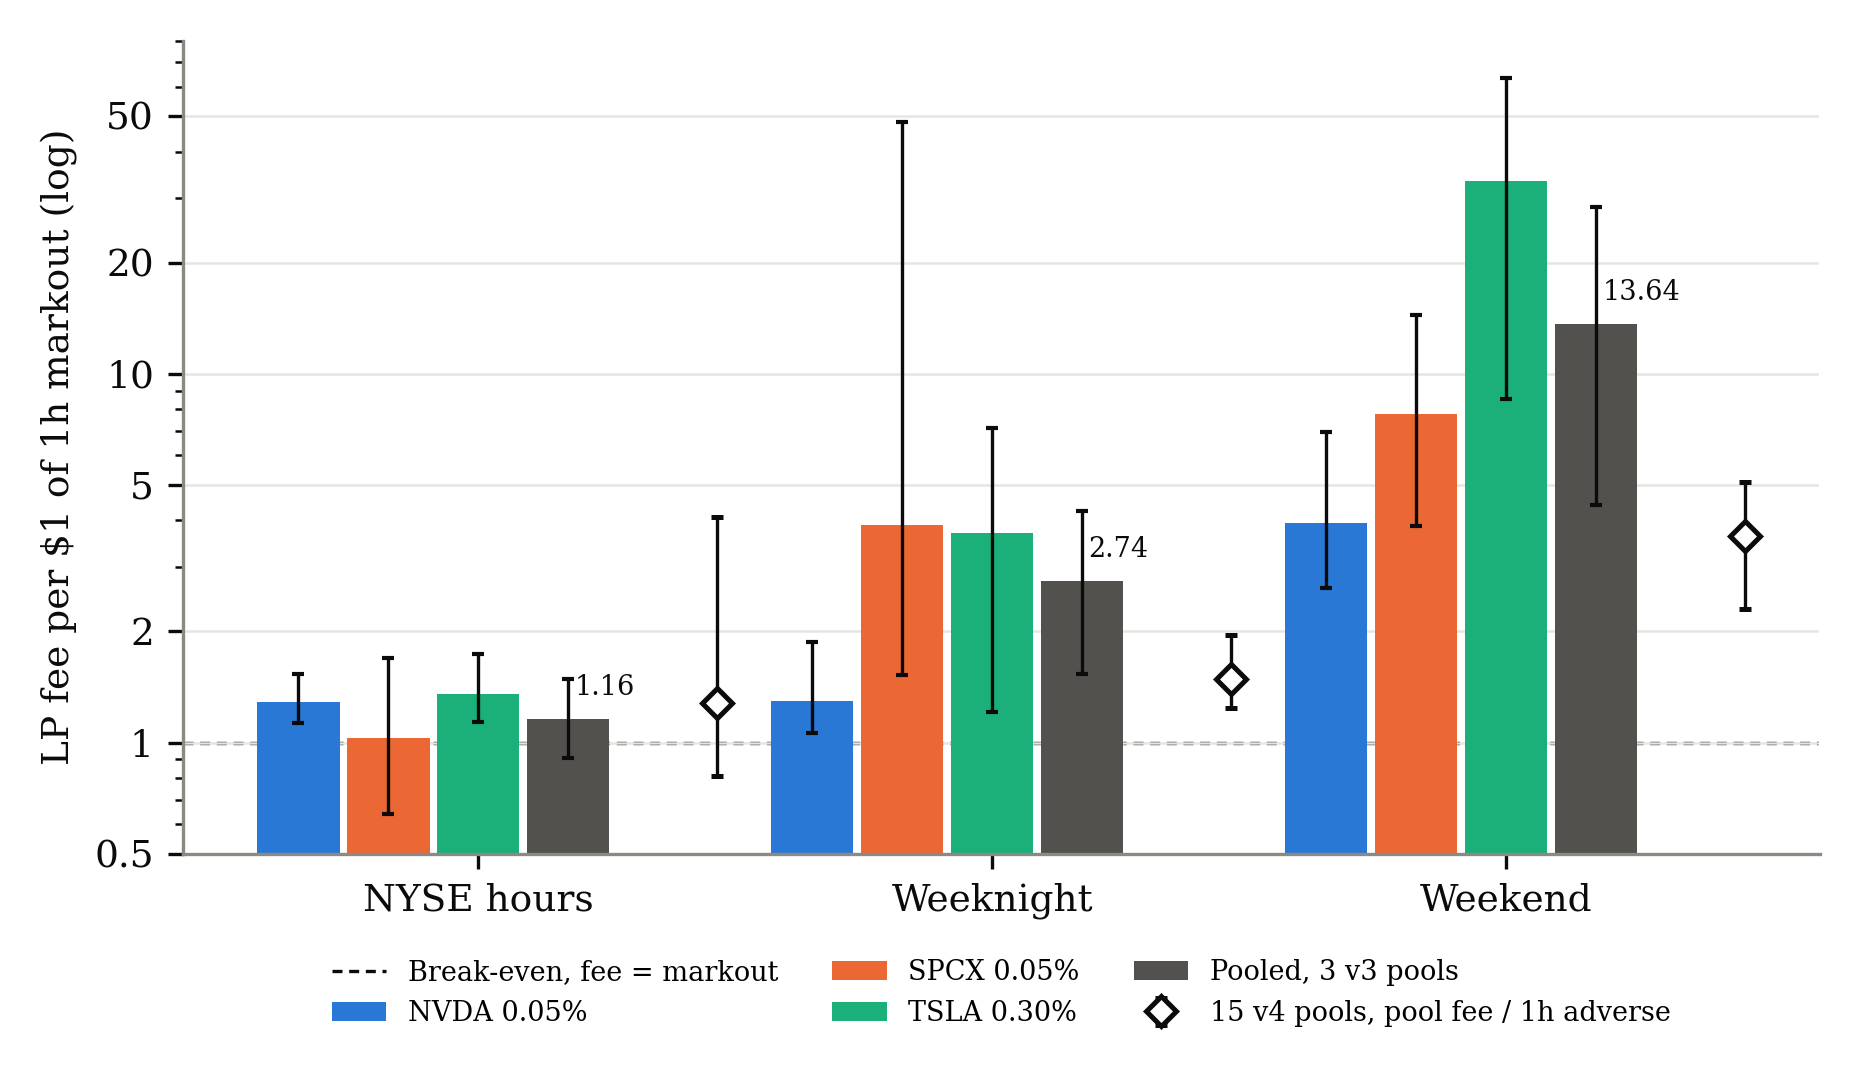
\includegraphics[width=0.92\linewidth]{figs/fig_sessions.png}
\caption{Fees earned per dollar of one-hour markout by session, log scale, with 90\% intervals. Bars: a \USD100K static $\pm2\%$ position under path accounting on each v3 pool (week-block bootstrap) and pooled across the three (2026-08-24 to 2026-10-17). Diamonds: pool-level fees over one-hour adverse selection on 15 v4 pools (day-block bootstrap, 2026-09-30 to 2026-10-16). Values below the dashed line mean the LP paid more to informed flow than it earned.}
\label{fig:sessions}
\end{figure}

\paragraph{What holds.} On every pool the weekend ratio exceeds the NYSE ratio, with a bootstrap probability that NYSE is below weekend of 1.000 on NVDA, SPCX and TSLA 0.30\%, and the weekend ratio is above the NYSE ratio in 22 of 23 pool-weeks (7 of 8 on NVDA, 8 of 8 on SPCX, 7 of 7 on TSLA 0.30\%). The pooled weekend ratio is 13.64 [4.41, 28.22] against 1.16 [0.91, 1.49] in NYSE hours, and the ordering holds under the flow bound (10.54 against 1.12), without SPCX (16.57 against 1.32), with equal pool weights (10.22 against 1.18) and at $\pm5\%$ (13.14 against 1.19). In basis points of absorbed volume, weekend toxicity is 1.27, 0.64 and 0.90 on the three pools against 3.88, 4.86 and 22.29 in NYSE hours, so the comparison does not depend on the fee tier.

\paragraph{What does not.} NYSE hours are not clearly the most toxic session. The bootstrap probability that NYSE is below weeknight is 0.518 on NVDA, 1.000 on SPCX and 0.864 on TSLA 0.30\%; only SPCX separates them. Fees do not fall below markout in NYSE hours on pooled data: the pooled NYSE ratio is 1.16 [0.91, 1.49] under path accounting, and it falls below one only for SPCX under the flow bound (0.94 [0.63, 1.46]). The earlier claim that fees cover markout less than one for one in NYSE hours is withdrawn; it rested on the mixed accounting, and under it NYSE ratios on SPCX and TSLA 0.30\% were 0.78 and 0.80, against 1.03 and 1.35 here. The weekend advantage also shrinks as volume falls. NVDA's weekend ratio is 1.19 and 1.38 in the last two weeks, against 7.09 and 22.57 in the first two, on weekend fees of \USD50 and \USD24 in the last two weeks, and in the last week NVDA's weekend ratio (1.38) is below its NYSE ratio (1.45).

\paragraph{Variance explains the markout.} Realised variance per hour of five-minute pool returns on NVDA is 2,424.7 bp$^2$ in NYSE hours, 697.0 on weeknights and 62.5 on weekends; the hourly markout of the position falls by a similar factor, so markout per unit of variance, relative to NYSE hours, is 0.94 and 1.48 on weeknights and weekends for NVDA, 0.51 and 0.77 for SPCX and 1.43 and 0.80 for TSLA 0.30\%. Markout per unit of variance varies by less than a factor of two across sessions, as loss-versus-rebalancing theory predicts. The weekend ratio is high because fees accrue on volume and weekend volume does not fall with variance: weekend hours are 30\% of the sample's hours and 17\% to 37\% of volume, against 62.5 bp$^2$ of hourly variance on NVDA, one thirty-ninth of the NYSE value.

\paragraph{Horizon.} Table~\ref{tab:horizons} reports the other horizons. The weekend lead holds at five minutes on every pool and at one hour, but it narrows with the horizon. At six hours NVDA's weeknight ratio is 0.80 and its NYSE ratio 1.05, so the weeknight is the most toxic session there, and marked to the next open NVDA's weeknight ratio is 0.61 against 1.64 for the weekend (whose interval, [0.68, inf], includes draws with a gain). On SPCX and TSLA 0.30\% weekend LPs gain on average when marked to the open (markout loss of $-$\USD455 and $-$\USD175), so the pooled weekend ratio at the next open, 38.78 [2.14, inf], reflects those two pools. The ordering of NYSE hours against weeknights flips with the horizon on NVDA, and the pooled weeknight ratio falls from 2.74 at one hour to 1.49 at the next open. A fee-over-markout ratio therefore needs its horizon stated; the one hour is the horizon fixed in our plan, and no horizon is privileged by the data.

\begin{table}[!tbp]
\centering
\caption{Fee per dollar of markout by horizon, \USD100K static $\pm2\%$, path accounting, fee-only. Off-hours swaps are marked to the pool price at 13:45 UTC on the next trading day in the last column; NYSE swaps keep the one-hour mark. Pooled rows carry 90\% week-block intervals from a separate bootstrap run, so the one-hour pooled interval differs in the third digit from Table~\ref{tab:pooled}.}
\label{tab:horizons}
\tabfit{t_horizons.tex}
\end{table}

\paragraph{Version 4 pools.} Table~\ref{tab:v4} reports 15 v4 pools at pool level. The weekend result replicates: the weekend has the highest fee over adverse selection in 6 of 7 tickers with weekend flow, and the pooled ratios are 1.28 [0.81, 4.08] in NYSE hours, 1.49 [1.24, 1.96] on weekday off-hours and 3.62 [2.30, 5.10] on weekends. The NYSE ranking does not: NYSE hours are the most toxic session for NVDA, META, MSTR and SPY only; weekday off-hours are for AAPL, SPCX and TSLA, and for CRCL the weekend is, with LPs gaining in NYSE hours. At the six-hour horizon weekday off-hours is the most toxic session (0.60 against 2.48 and 3.04), and marked to the next open the three sessions are indistinguishable (1.28, 1.36 and 1.19). In basis points of volume the fee is 16.8, 8.0 and 2.7 across the three sessions, because the NVDA 0.01\% pool supplies most of off-hours volume, so pooled ratios compare different pool mixes. The sample includes dynamic-fee session hooks (FablesRWA, SessionFeeHook), so part of the v4 fee profile is those hooks' own schedules; the 10 hookless pools give 1.25, 1.53 and 3.82 at one hour.

\begin{table}[!tbp]
\centering
\caption{Fifteen v4 Stock Token pools, 2026-09-30 to 2026-10-16, pool-level fees and adverse selection. Top: by ticker, one-hour horizon. Bottom: dollar-weighted fee over adverse selection by horizon with 90\% day-block bootstrap intervals, then equal pool weights and the 10 hookless pools. ``Gain'' marks adverse selection at or below zero.}
\label{tab:v4}
\tabfit{t_v4tick.tex}

\vspace{6pt}
\tabfit{t_v4pool.tex}
\end{table}

\paragraph{Why the weekend is benign, and what is not shown.} On weekends the NVDA pool sat a median 44.4~bp from the stale Chainlink price but 4.1~bp from the 24/7 perpetual; for TSLA 0.30\% the figures are 52.8 and 11.8~bp, and for SPCX 25.7 and 14.0~bp. In the regular session the NVDA pool sits closer to Chainlink (15.5~bp) than to the perpetual (18.2~bp), which is partly the half-hour lag of the interpolated hourly candle. These medians show co-movement, not direction. We have not run a lead-lag test, and the data cannot say whether arbitrage carries the perpetual into the pools or the perpetual follows the pools. The weekend mark and oracle of the perpetual are not modelled here either.

Flow composition is not benign by construction. On TSLA 0.30\% the weekend has 103,418 swaps against 40,077 in NYSE hours and \USD13.34M of volume against \USD12.82M, 67.0\% of weekend volume goes to one recipient, and 82.0\% of weekend volume is offset by the same recipient on the same day against 65.4\% in NYSE hours, which looks like bot or volume-farming flow. Dropping each session's largest recipient leaves the ordering intact (weekend 16.69 against NYSE 2.09 and weeknight 3.39), as does dropping the ten largest (11.40, 3.37 and 3.80). The weekend result thus holds with the dominant actor removed, but the profile describes the flow these pools received and not the calendar alone.

\subsection{Hours-aware ranges}\label{sec:res:ranges}

Table~\ref{tab:strategies} reports net-versus-hold and edge APRs under path accounting, the pool-impact and \USD1M variants, and the flow bound for edge. Table~\ref{tab:prereg} applies the pre-specified claim to every cell of capital, cost model and metric.

\begin{table}[!tbp]
\centering
\caption{Strategy returns, APR points. Edge is fees minus one-hour markout loss minus rebalancing cost. Net versus hold is not reported under flow accounting, whose per-swap inventory path and end-of-window value do not come from one counterfactual. A: full range; B2, B5, B10: static $\pm2\%$, $\pm5\%$, $\pm10\%$ recentred daily; C: hours-aware; D: C with weekend and stale-feed withdrawal. TSLA 0.05\% pays impact on a pool smaller than the position in Panels B and D. 2026-08-24 to 2026-10-17 (TSLA 0.05\% from 2026-09-14).}
\label{tab:strategies}
\tabfit{t_strategies.tex}
\end{table}

\paragraph{The pre-specified claim is not refuted, and not supported.} Under path accounting with fee-only rebalancing costs, C earns more than the best static range on NVDA (edge 36.8 against B2's 28.4), on TSLA 0.30\% (181.3 against 142.3) and on SPCX (92.2 against 75.9), and its net versus hold passes the bar on NVDA (25.0 against B5's 14.2) and TSLA 0.30\% (186.8 against B2's 137.4). The claim is met in the two fee-only cells and in none of the four pool-impact cells (Table~\ref{tab:prereg}); under the flow bound it is met in one of four edge cells. The verdict reverses with the rebalancing cost because C rebalances at every session change (114 times on NVDA against 54 for a daily static range) and pays impact each time: at \USD1M under pool-impact costs C's edge is $-52.4$, $-364.9$ and $-193.9$ APR on NVDA, TSLA 0.30\% and SPCX. The statement of the earlier version that the claim fails on 0 of 3 tokens was an artefact of the mixed accounting and is withdrawn.

\begin{table}[!tbp]
\centering
\caption{The pre-specified claim in each cell: C or D earns at least 5 APR points and beats the best static range by at least 2 points on at least 2 of 3 tokens. Net versus hold is not defined under flow accounting (Table~\ref{tab:strategies}).}
\label{tab:prereg}
\tabfit{t_prereg.tex}

\vspace{6pt}
\caption*{Paired week-block bootstrap, \USD100K fee-only: C minus the best static range of the full window (B2 for edge on all tokens; B5 on NVDA and B2 on TSLA 0.30\% and SPCX for net), 90\% intervals. Point estimates are weekly-weighted and differ slightly from Table~\ref{tab:strategies}.}
\tabfit{t_boot.tex}

\vspace{6pt}
\caption*{Decomposition under path accounting, \USD100K, fee-only, APR points: edge is fees minus markout minus cost; beta is the price-level term; $F-C+\mathrm{LVR}$ is the alternative, convexity-based measure.}
\tabfit{t_decomp.tex}
\end{table}

\paragraph{The margin is not precise.} The paired intervals for C minus the best static range include zero on every token for edge, $+8.3$ [$-1.5$, $+18.3$] on NVDA, $+40.4$ [$-5.8$, $+88.4$] on TSLA 0.30\% and $+17.0$ [$-28.0$, $+59.8$] on SPCX, with the 2-point bar cleared in 85\%, 91\% and 71\% of draws; for net the interval excludes zero on NVDA and TSLA 0.30\% against the best static range of the full window, and includes it against the best static range in each draw. Under the flow bound the NVDA margin is $+7.0$ [$-1.8$, $+16.0$] and TSLA 0.30\% is $-12.9$ [$-27.1$, $-0.6$].

\paragraph{The calendar is not what pays.} In the placebo, the real calendar is above the mean of the shuffled calendars in 35 of 64 cells, and the share of shuffles at or above the real result runs from 0.00 to 0.96. The pre-named cell has exact permutation $p$ of 0.743 on NVDA (real 25.0 against a shuffled mean of 35.7), 0.178 on SPCX (59.9 against 41.7), 0.347 on TSLA 0.30\% (186.8 against 173.7) and 0.208 on TSLA 0.05\% (100.7 against 77.9). Eight cells reach $p \leq 0.05$, all under fee-only costs and all on SPCX or TSLA 0.05\%. Randomly assigned session labels match C's gain over static ranges in most cells, so C's edge is not attributable to the calendar; part of it may come from running a narrower range for part of the week, which we did not separate. The earlier reading that the real calendar lies below the shuffled mean in 64 of 64 cells and that an inverse schedule wins is withdrawn: both were computed under the mixed accounting, and the inverse schedule was found after the data were seen.

\paragraph{Price level and fees.} A two-sided range centred on the price holds about half its value in USDG, and the tokens moved $-2.12\%$ (NVDA), $-3.35\%$ (TSLA 0.30\%) and $+7.23\%$ (SPCX) over the window. The beta term is nevertheless negative for every static range on every pool (B2: $-87.1$, $-100.8$ and $-79.7$ APR points), so static ranges beat holding through fees net of markout, convexity and cost, in spite of the price level and not because of it. SPCX, whose price rose, is the clear case: B2 beats holding by 93.4 points. We rank by edge and report $F-C+\mathrm{LVR}$ beside it, since the two differ by up to 67 points on NVDA B2 (28.4 and 95.4).

\paragraph{Monday open versus the weekend before it.} Designs that charge the weekend most treat the reopening as the main LP loss. Table~\ref{tab:mondayhours} splits each of seven Mondays with an open (the Labor Day Monday excluded, since the exchange was shut) into the weekend, the Monday pre-open and the open hour, for the static $\pm2\%$ position under path accounting. The open hour loses on NVDA ($-$\USD427) and TSLA 0.30\% ($-$\USD2,377) and gains on SPCX (+\USD1,683), and in each token one Monday supplies 66\% to 85\% of the open-hour markout (one Monday, 2026-10-05, accounts for \USD2,555 of SPCX's \USD3,023). The weekend before earns \USD706, \USD1,136 and \USD7,305 net. The reopening loss is real and, on NVDA and TSLA 0.30\%, smaller than the preceding weekend's net earnings, but it rests on a few Mondays.

\begin{table}[!tbp]
\centering
\caption{Net LP earnings (fees minus one-hour markout, \USD) of a \USD100K static $\pm2\%$ position in the weekend (Friday 20:00 to Monday 00:00 UTC), the Monday pre-open (00:00 to 13:30) and the Monday open hour (13:30 to 14:30), summed over seven Mondays with an open, with volume in \USD M in parentheses; and the share of the open-hour markout supplied by the largest single Monday and the number of Mondays with negative open-hour net. Path accounting, fee-only. The weekend before the first Monday (2026-08-24) precedes the window and is excluded from the weekend total.}
\label{tab:mondayhours}
\tabfit{t_mondayhours.tex}
\end{table}

\subsection{Session-priced and oracle-gap fees out of sample}\label{sec:res:fees}

Table~\ref{tab:elast} reports the fee elasticity of volume. The cross-section across 14 pools gives 0.87 (s.e.\ 0.13) with a depth control and 0.63 without one; fee and depth are nearly uncorrelated (0.08), yet the control moves the estimate. Leaving out each pool in turn gives 0.72 to 0.94. The within-pair estimate is 0.74 as published, and 0.78 [0.67, 0.89] once the duplicated NVDA Fables pair is dropped. It is not robust to the volume floor: it is 0.67 at a floor of \USD2,000, 0.78 at \USD500, 1.05 at \USD100 and 1.58 at \USD0. Dropping hours in which a pool trades little removes exactly the hours in which a high fee may have driven volume away, which biases the estimate toward the threshold of one on which every fee result below turns, and we cannot place $\varepsilon$ on either side of one with confidence. Session by session the cross-section gives 0.81, 0.81 and 0.88, but the differences have pool-cluster intervals of about $\pm0.4$ to $\pm0.5$ (weekend minus NYSE $+0.06$ [$-0.36$, $+0.53$]), so the data do not show that elasticity is equal across sessions; they cannot exclude a session difference of the size at which a session schedule would matter. Elasticity is estimated mostly on v4 pools and applied to v3 pools.

\begin{table}[!tbp]
\centering
\caption{Fee elasticity of pool volume, 2026-10-01 to 2026-10-16. Intervals are wild cluster bootstrap over 16 days (within-pair rows), the leave-one-pool-out range (cross-section, marked a) and pool-cluster bootstrap (session differences, marked a). The volume floor drops hours in which either pool of a pair trades less.}
\label{tab:elast}
\tabfit{t_elast.tex}
\end{table}

\paragraph{The test is uninformative at elasticity below one.} At $\varepsilon = 0.8$, every session chooses the 35~bp cap in calibration on every token, the session schedule collapses to the best flat fee, and its gain over that fee is 0.00 APR points on both splits and on all three tokens (Table~\ref{tab:fees}). By equation (3) this is the algebraic consequence of the model and the cap, not an observation: no schedule could have met the pre-specified 5-point bar at any $\varepsilon<1$. The same holds at $\varepsilon=0.6$ and $1.0$. At $\varepsilon = 1.5$ and $2.0$, where an interior optimum appears, the session schedule has no consistent sign: its gain over the flat fee is $-1.16$, $-26.17$ and $+1.95$ at 1.5 and $-4.29$, $-15.79$ and $-27.99$ at 2.0 on NVDA, SPCX and TSLA 0.30\%. Only the second case is informative, and only for one elasticity shared by all sessions. The calibrated model also leaves its domain: the NVDA oracle-gap schedule at $\varepsilon=2.0$ gains 295.57 points, and the TSLA 0.30\% one loses 2,862.85.

\begin{table}[!tbp]
\centering
\caption{Out-of-sample fee test for a \USD100K static $\pm2\%$ position (path accounting), edge in APR points on the test half, schedules calibrated under response (ii) with $\varepsilon = 0.8$ unless stated and capped at 35~bp. Gain rows are differences from the best flat fee calibrated on the same half. Responses: (i) none, (ii) constant elasticity, (iii) benign flow only.}
\label{tab:fees}
\tabfit{t_feetest.tex}
\end{table}

\paragraph{The oracle-gap term is not stable.} Adding the oracle-gap term helps NVDA by 9.78 points under (ii) on the forward split and 52.10 on the reverse split, and the gain is $-8.03$ and $-166.43$ under (i) and $-0.89$ and $-18.38$ under (iii). It hurts SPCX under every response and both splits ($-14.02$ and $-6.43$ under (ii)) and TSLA 0.30\% on the forward split ($-49.30$). On the forward split the fee schedule charges 1~bp on weeknight toward-oracle flow on NVDA and 35~bp elsewhere; the gain then comes from raising that bucket, whose markout favours the LP ($-$\USD231 of loss), by $(0.2)^{-0.8}$, a volume inflow extrapolated below the lowest fee observed on the chain (1.25~bp). With a floor at 1.25~bp the NVDA gain is 5.09 and the TSLA 0.30\% loss is 27.92. With the calibration in the half that contains the elasticity window (reverse split) the elasticity is no longer estimated inside the test half. The flow bound gives $+9.32$, $-25.66$ and $-4.31$.

\paragraph{Toxicity by oracle direction follows the session.} Table~\ref{tab:direction} reports pool-level one-hour markout of swaps that move the pool toward or away from the Chainlink price, gross of the LP fee; negative values are adverse selection. An earlier version reported the net-of-fee figures, which on TSLA 0.30\% mostly show the 30~bp fee. On NVDA, toward-oracle flow costs the LP 5.50~bp in NYSE hours and earns it 6.00~bp on weeknights; at the same feed age of 0 to 30 minutes the sign is $-7.33$~bp in NYSE hours and $+12.59$~bp on weeknights (Table~\ref{tab:age}). The sign therefore follows the session and not the age of the feed. SPCX does not follow NVDA, and on TSLA 0.30\% every cell is adverse. Calibrating a fee per direction, session and token on four weeks fits a seven-cell table to 27 days: the NVDA weeknight toward-oracle cell is cheapest in calibration, the SPCX NYSE toward-oracle cell is cheapest in calibration and toxic over the full window ($-9.68$~bp gross), and a median Chainlink update moves the price by 53 to 54~bp, so the grid of gap thresholds ($\vartheta$ of 0, 15 and 30~bp) lies inside the feed's own update threshold. We drop the earlier mechanism that toxic flow reverses as the feed ages.

\begin{table}[!tbp]
\centering
\caption{Pool-level one-hour markout by oracle direction, basis points of volume, LP view gross of the pool fee (net of fee in parentheses), full window. Negative gross values are adverse selection. Below: NVDA by Chainlink feed age, gross of fee.}
\label{tab:direction}
\label{tab:age}
\tabfit{t_direction.tex}

\vspace{6pt}
\tabfit{t_age.tex}
\end{table}

\paragraph{The fee level is a model-implied hypothesis.} Moving from the pool's own tier to 35~bp raises edge on every token under every response and both splits (forward, 88.81, 220.61 and 13.75 points under (ii); 482.97, 982.86 and 19.09 under (i); 38.30, 77.94 and 3.59 under (iii)), but the size varies by an order of magnitude across responses. For NVDA and SPCX that is an extrapolation to seven times the 5~bp tier, outside the fees from which the within-pair elasticity is identified (standard deviation of the log fee 0.34 to 0.39), and the counterfactual is not available to an LP: the NVDA v4 0.30\% pool traded \USD2.60M at a median active liquidity of $4.86\times10^5$ while the v3 0.05\% pool traded \USD99.77M at $4.71\times10^6$ in the elasticity window. We read the sign and not the size, and we treat it as a hypothesis, not as a measured effect. A model-free comparison of the same token in two tiers needs positions small relative to both pools, and the TSLA 0.05\% pool is too shallow for it.

\subsection{Weekend price discovery}\label{sec:res:monday}

Table~\ref{tab:monday} and Figure~\ref{fig:monday} report the Monday-open test. Against a stale Friday close, whose mean absolute error at the Monday open is 136.9~bp, a perpetual price read on Sunday at 16:00 UTC reduces absolute error by 3.7\% [$-$4.6, 12.2] in the pooled leave-one-weekend-out test, and mean squared error by 16.4\% [2.1, 28.6]; the correlation between the perpetual move and the gap is 0.41. Over the 12 weekend read times the mean absolute-error reduction is 3.5\% [$-$4.2, 8.6] and the maximum is 7.3\%, so Sunday 16:00 sits in the middle of a profile that runs from $-$3.7\% to 7.3\% in absolute error, and the weekend reductions are individually indistinguishable from zero in absolute error. The reduction is 14.8\% [2.1, 25.4] on Monday at 00:00, after US index futures reopen on Sunday at 22:00 UTC and the overnight session opens, 36.5\% [23.0, 46.3] at 08:00 in the pre-market, and 69.3\% [64.0, 73.4] at 13:00 (91.2\% in squared error), half an hour before the open. Adding holiday weekends (29 weekends, 203 ticker-weekends) leaves Sunday 16:00 at 2.5\% [$-$4.4, 8.9].

\begin{table}[!tbp]
\centering
\caption{Reduction in Monday-open error from a perpetual-futures price read at the stated time (UTC), relative to the stale Friday close. Leave one weekend out, 24 plain Friday-to-Monday weekends per ticker from 2026-03-23; the per-ticker rows are mean absolute error. Pooled rows carry 90\% weekend-block bootstrap intervals that re-estimate the slope in each draw. The control pairs each ticker's gaps with its perpetual moves from another weekend (23 circular shifts) and reports the mean and maximum over shifts.}
\label{tab:monday}
\tabfit{t_monday.tex}
\end{table}

\begin{figure}[!tbp]
\centering
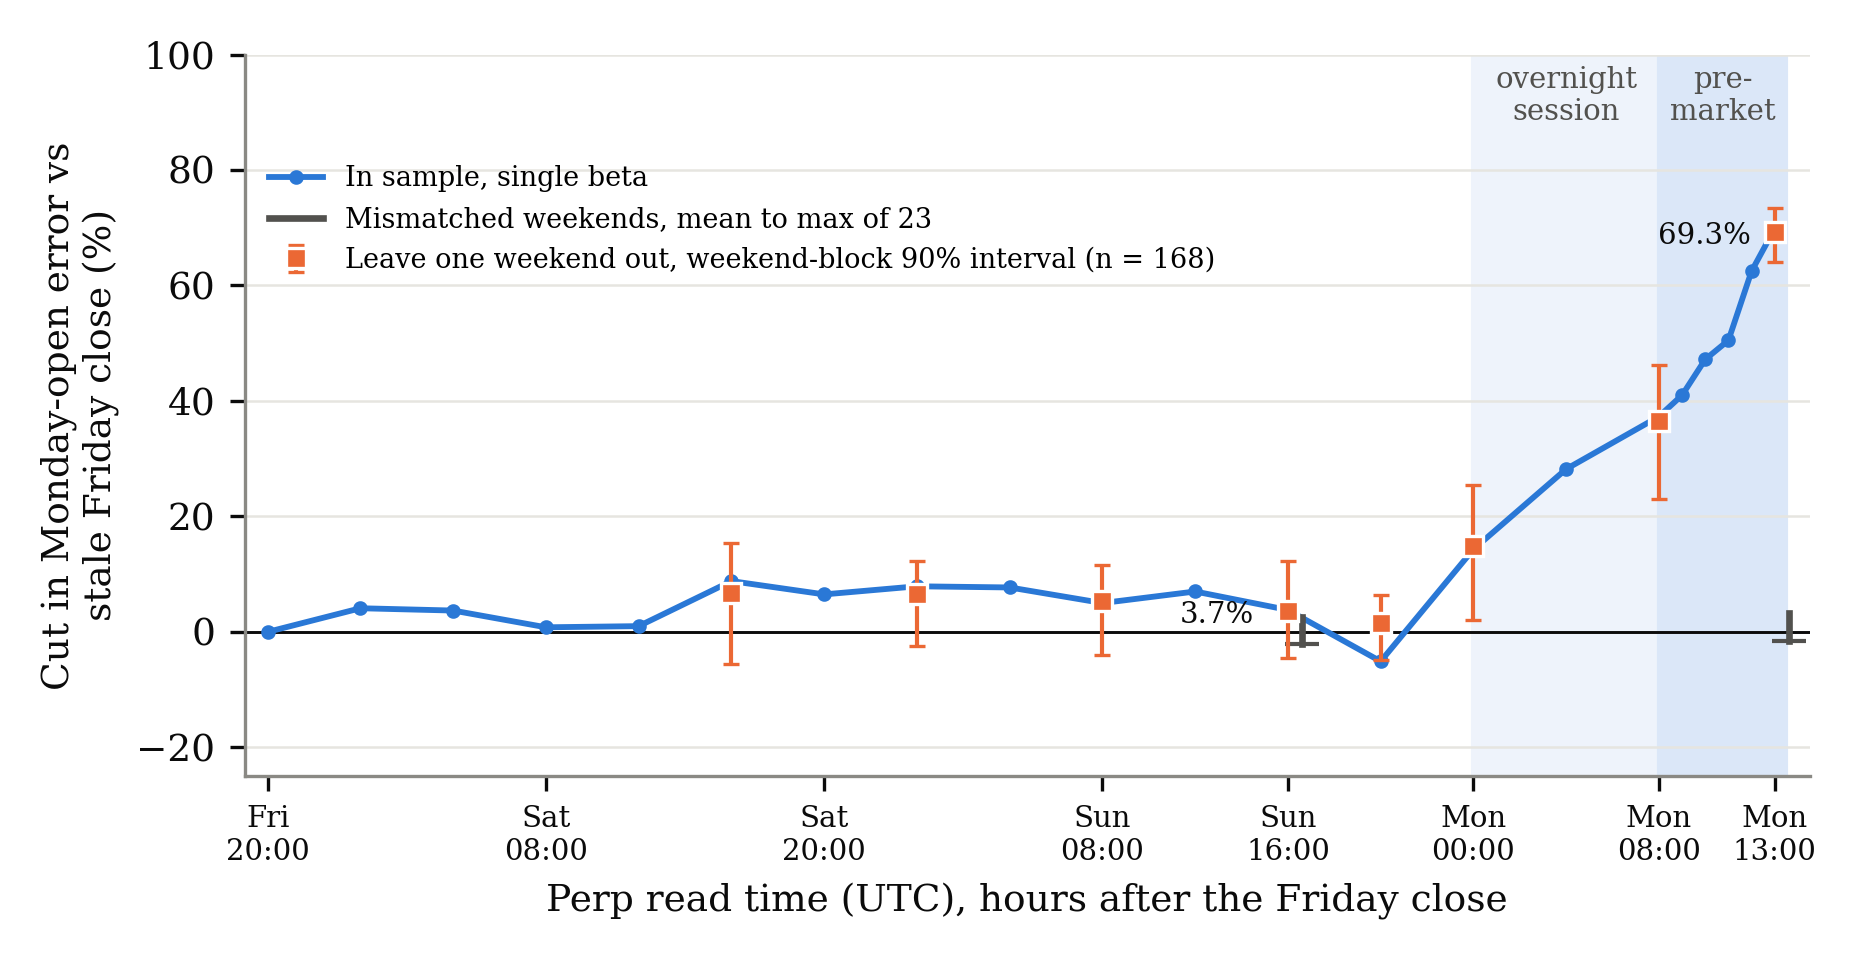
\includegraphics[width=0.92\linewidth]{figs/fig_monday.png}
\caption{Reduction in Monday-open absolute error from a perpetual price read at each hour after the Friday close. Line: in-sample fit with a single pooled coefficient. Squares with bars: leave-one-weekend-out estimates with 90\% weekend-block intervals at eight read times. Grey: the mismatched-weekend control (mean to maximum over 23 shifts). Shading marks the Monday overnight session and the pre-market.}
\label{fig:monday}
\end{figure}

The weekend perpetual move therefore carries detectable but small information about the Monday gap: the real pairing beats all 23 mismatched pairings at Sunday 16:00 (control mean $-2.1\%$, maximum 2.6\%), a one-sided permutation $p$ of about $1/24$ and so a detectable correlation, while the gain in absolute error is 3.7\% with an interval that spans zero. Most of the information arrives with the Monday overnight and pre-market sessions, consistent with the convergence pattern in \citet{agarwal2026bitquery} and the decomposition of \citet{cha2026nest}. The result is for this perpetual: we do not model how the venue forms its weekend mark, and a different venue or an index product may carry more. For the LP this is the price-side view of Section~\ref{sec:res:session}: a weekend fair-value oracle built on this perpetual would add little to what the deep pools already trade at, and the information an LP loses to arrives mostly after the weekend.

\section{Implications for LP vault design}\label{sec:design}

The results translate into a small set of design rules for an LP product that takes a Stock Token deposit and provides liquidity on the holder's behalf.

\begin{enumerate}[leftmargin=*,itemsep=3pt]
\item \textbf{Choose the pool and fee tier by measured edge, on swaps the selection did not see.} Pools and tiers differ as much as sessions do (Table~\ref{tab:session}), and selection on in-sample edge can pick a pool whose held-out edge is near zero (Appendix~\ref{app:product}). Whether a higher fixed tier would raise edge is a hypothesis of the volume model, not a measured effect (Section~\ref{sec:res:fees}).
\item \textbf{Keep ranges static across sessions and recentre once a day unless rebalancing costs only the fee.} The hours-aware strategy clears its bar only when rebalances pay the pool fee alone; with pool impact it loses to static ranges (Table~\ref{tab:prereg}), and its edge is not attributable to the calendar.
\item \textbf{Stay in the market on weekends.} The weekend ratio exceeds the NYSE ratio on every pool and in 22 of 23 pool-weeks, and withdrawing on weekends (strategy D) gives up the session with the least toxic flow per dollar traded.
\item \textbf{Treat the oracle as a valuation input with a calendar.} A 24/5 feed is hours old on weeknights and roughly a day or more old on weekends. A vault that values shares with it must bound staleness, cross-check the pool's time-weighted and spot prices, and handle the weekend explicitly. A fee or range keyed to the distance from the oracle changed sign across our splits and is not supported.
\item \textbf{Account for the stablecoin half.} A $\pm5\%$ range centred on the price holds 48.8\% of its value in the token at entry, so 51.2\% of a token-only deposit becomes USDG, and comparisons with holding are dominated by the price level. A holder who wants the full token exposure can restore it with a long perpetual position; over our window the Hyperliquid xyz funding paid by longs averaged 5.5\% APR on NVDA, 6.8\% on TSLA and 1.7\% on SPCX (1,296 hourly prints each), which sets the cost of that hedge.
\end{enumerate}

\section{Scope of the evidence}\label{sec:scope}

The v3 results come from one 54-day window in which volume fell steadily, and the intervals rest on eight weekly blocks (one partial) and 24 weekends. The session profile could differ in a regime of rising volume or around earnings and macro events. Dollar-weighted pooled statistics are dominated by NVDA and SPCX (SPCX supplies 55\% of pooled NYSE markout and listed on 2026-06-12), and TSLA 0.30\% is small. The v4 sample covers 15.95 days and two weekends inside the v3 window, so it is a second set of pools and not a second period, and its pool list is chosen on volume. The Monday-open test uses seven single stocks; index products, whose futures reopen on Sunday evening, may carry more weekend information, and the Monday-open-hour comparison rests on seven Mondays.

The replay engine uses the active liquidity reported at each swap rather than the full tick map, does not model just-in-time liquidity or same-block mints and burns, and does not simulate trading halts; its two accounting bounds are first order and neither re-simulates the price path. The one-hour markout uses the same pool's price as its reference, so a pool that lags the exchange at the open understates adverse selection there; we have not measured markouts against an external 24/7 price, which a minute-level perpetual series would allow. Strategy C centres on the Chainlink price, which updates every 12 to 27 minutes with a 53 to 54~bp median move, and we have not tested a variant centred on the pool's time-weighted price. The fee test's volume response is a constant-elasticity model fitted on 16 days and 14 pools in which LP supply does not respond to the fee, and the elasticity was estimated inside the half used as the test half in the forward split. The placebo cells share data and are not independent. The decisions fixed in advance are those listed in Section~\ref{sec:method}; the pre-specification has no external timestamp. Every result in the paper is regenerated by a script in the replication package (Appendix~\ref{app:repro}).

\section{Conclusion}\label{sec:conclusion}

In a 24/7 AMM whose reference market closes, LPs lose least to informed flow on weekends. On Robinhood Chain's Stock Token pools, a static position earns 13.64 [4.41, 28.22] dollars of fees per dollar of one-hour markout on weekends against 1.16 [0.91, 1.49] in NYSE hours, with the weekend ahead of NYSE hours in 22 of 23 pool-weeks and under both finite-position accounting bounds. The margin narrows when weekend swaps are marked to the next open, NYSE hours cannot be separated from weeknights on two of three pools, and fees do not fall below markout in NYSE hours. Markout per unit of realised variance is within a factor of two across sessions, and the weekend ratio is high because fees follow volume while information follows variance. Weekend perpetual prices carry detectable but small information about the Monday open, which arrives mostly after US futures reopen.

The calendar does not, on this evidence, make a better strategy. An hours-aware range beats static ranges at point estimates only when rebalancing is cheap, with margins whose intervals include zero and a gain that random session labels match. Session fee schedules cannot be tested at the elasticity we measure, because they collapse to the fee cap by construction there, and an oracle-gap fee changes sign with the sample split. What the data do establish is a session profile that is robust across weekends, a method for reporting it with intervals and accounting bounds, and a corrected engine on which the next tests can be run.

\FloatBarrier
\bibliographystyle{plainnat}
\bibliography{refs}

\clearpage
\appendix
\section{Fee-taking hooks and an in-swap cap}\label{app:hooks}

This appendix concerns traders and routers that choose pools by their displayed fee, not LP deposits: a take through a hook's swap-side return deltas reduces what a swapper receives and does not touch an LP's deposit, and the LP vault of Appendix~\ref{app:product} sits in v3 pools, which carry no hooks. LP-side risks live in add- and remove-liquidity deltas and in fee diversion, which the cap below does not bound.

\paragraph{Realised take.} In the 49-hour census, 42.8\% of the 3,183,184 v4 swaps ran through pools with a hook, and 26.7\% through pools whose hook holds a return-delta permission, which allows a take that the Swap event's fee field does not show. Only 3.1\% of swaps carry an event-visible fee of 5\% or more. One family of 36 hooks shares a runtime with an immutable \texttt{feeBps} of 1000 and sits on pools with a 1\% fee. Over the census its pools executed 25,504 swaps (14,758 buys and 10,746 sells, 0.80\% of all swaps) with \USD4,583,144 of gross value, and the hooks took \USD458,314, 10.00\% of gross, on top of the 1\% pool fee; this figure multiplies the immutable \texttt{feeBps} by event volume for all 25,504 swaps and is computed from code and events, not observed as a transfer on each swap. Dollar values for ETH-paired pools use one Chainlink ETH/USD read of \USD2,439.28 at the window midpoint. The take is public in the hook's bytecode and some interfaces show it (GMGN displays a total-tax figure for these tokens, 11\% for the 10\% family); what the pool's Swap event does not show is a take through return deltas.

For the Pons fee hook we join Swap events to the hook's own \texttt{HookFeeCollected} events by transaction and pool over blocks 90,230,000 to 90,239,999 (about 17 minutes). On the 488 fee events paid in native ETH from single-swap transactions, 474 of which are sells, the Swap event's LP fee is zero in 488 of 488, while the hook's fee plus tax as a share of the ETH leg has a 10th percentile of 1.00\%, a median of 3.00\%, a 90th percentile of 3.00\%, a 99th percentile of 4.00\% and a maximum of 7.00\%. The meaning of \texttt{taxAmount} is read from the contract's ABI field name. This is one 17-minute window dominated by sells, and the earlier Bitquery census measured a median 1\% against a displayed 0\% for the same hook family \citep{bitquery2026hooks}. These are memecoin pools and not Stock Token pools, though the same PoolManager and routers serve both. Slippage bounds, quote simulation (which executes the hook) and router allowlists already limit the exposure, and Uniswap's own router allowlist includes the Pons hook.

\paragraph{An in-swap cap.} An abstract hook base, \texttt{CappedTakeHook}, wraps a builder's \texttt{beforeSwap} and \texttt{afterSwap} logic. In \texttt{afterSwap} it computes the take the builder's code returned on the specified leg, on the unspecified leg and through any dynamic LP fee, rounds each leg up, and reverts with \texttt{TakeExceedsCap} when the total exceeds an immutable \texttt{maxTakeBps}. A write-once \texttt{CapRegistry} records each hook's declared cap from its constructor. Because v4-core skips hook callbacks when the hook itself calls the pool, the base reads the pool's price, tick and active liquidity before and after each builder callback and reverts on any change.

We run 26 tests on a Foundry fork of Robinhood Chain against the deployed PoolManager, with new tokens, pools and hooks per test. With a hook that takes 3\%, a cap of 250~bp reverts every one of 200 swaps and a cap of 300~bp passes every one of 200; these are repetitions of a deterministic construction, so they are unit-test passes and not a rate, and the fuzz runs (256 of 256) are the evidence about input coverage. One basis point either side of the cap behaves correctly in 60 of 60 swaps, a 50~bp dynamic fee against caps of 49 and 50~bp and a 250~bp take split across three paths also split correctly 60 of 60, and the computed take equals the trader's loss against an identical pool without a hook to the wei on the Pons-shaped and dynamic-fee paths (64 swaps each). For exact-output swaps that take on the specified leg the aggregate is off by up to 0.9\%, a worst-case understatement of 2.80~bp against the cap, and exact-output swaps below about 100 wei pass (50 wei passes, 99 wei and above revert). Without the nested-state guard, a hook that trades against its own pool costs the trader 385~bp while the base reports a take of zero; with the guard both directions revert. The overhead is 25,174 to 25,263 gas per swap against an uncapped hook with the same permissions as the Pons hook, 22,961 to 23,050 against an uncapped hook with the base's own permission bits, and 22,721 on the dynamic-fee path, of which the guard accounts for 6,833, under Foundry's gas schedule on a fork. The cap binds only hooks that inherit the base, and a registry entry is a declaration: a hook can register a cap without inheriting the base, so a router needs a codehash or factory attestation before it can rely on one.

\section{Application: the evidence engine in a vault}\label{app:product}

The author develops Uptick, whose \texttt{StockVault} is an ERC-4626 vault per Stock Token that holds one Uniswap v3 position recentred daily at the NYSE open around the Chainlink price and keeps it in the pool through the weekend; the vault contract uses no hook. The contracts and the keeper's evidence engine are implemented and tested on a local fork of chain 4663, and we report engine results, not deployed returns. The engine is the replay engine of Section~\ref{sec:method} with the earlier mixed accounting, and the bias described there applies to its numbers: it penalises thin pools when selecting by edge.

Its 30-day replay of a \USD100K $\pm5\%$ NVDA position recentred daily at the open, under pool-impact costs (509,293 swaps, \USD348.7M of volume), shows a fee APR of 40.56 against a markout APR of 30.90 and a cost APR of 4.62, an edge of 5.04 APR, and net versus hold of $-9.01$. The engine's own held-out check on the pool it selected, which calibrates on 2026-09-17 to 10-02 and tests on 10-02 to 10-17, returns an edge of 10.9 APR on the calibration half and $-0.42$ on the test half. Every value-in and value-out path is gated on feed freshness and on agreement between the feed, the pool's time-weighted price and its spot price; with a 25-hour staleness bound and a weekend feed age of 24.6 hours at the median and 61 hours at the 90th percentile, the gate is closed for cash deposits and withdrawals for much of every weekend, while redemption in kind of both tokens, which needs no price, stays open. The repository also holds a separate v4 hook prototype with a session fee and an oracle-gap surcharge; the vault does not use it, and Section~\ref{sec:res:fees} reports why the data do not motivate it.

\section{Reproduction map}\label{app:repro}

Every table cell of Section~\ref{sec:results} is generated by \texttt{revision/scripts/make\_tables.py} from a log file, and the generated ledger \texttt{revision/claims\_generated.md} lists each cell with the file and line it was read from. Other numbers in the text are in the claim ledger distributed with the paper (\texttt{claims.md}, sections R and the earlier sections). Cached swap pulls and reference data were used for every re-run; the chain was queried only for the checks of Appendix~\ref{app:product} and the fork tests of Appendix~\ref{app:hooks}.

\begin{center}
\small
\begin{tabular}{>{\raggedright\arraybackslash}p{4.4cm}>{\raggedright\arraybackslash}p{2.2cm}>{\raggedright\arraybackslash}p{8.4cm}}
\toprule
Result & Ledger IDs & Script \\
\midrule
Table~\ref{tab:data}, interpolation error & A1 to A3, A5, A8, R1 & \texttt{run.py}, \texttt{pooled\_sessions.py}, \texttt{revision/scripts/interp\_error.py} \\
Engine tests, mutations, legacy check & A7, R2 & \texttt{test\_engine.py}, \texttt{mutation\_check.py}, \texttt{engine.py} with \texttt{SHARE=path|flow|mixed} \\
Tables~\ref{tab:session}, \ref{tab:pooled}, \ref{tab:horizons}, Fig.~\ref{fig:sessions} & R3 to R6 & \texttt{revision/scripts/sessions.py} (\texttt{--horizons}) \\
Flow composition & R7 & \texttt{revision/scripts/flow\_composition.py} \\
Table~\ref{tab:v4} & R8 & \texttt{revision/scripts/v4\_sessions.py} \\
Tables~\ref{tab:strategies}, \ref{tab:prereg}, placebo & R9 to R12 & \texttt{run.py}, \texttt{revision/scripts/strategy\_tables.py}, \texttt{strategy\_boot.py}, \texttt{shuffle.py}, \texttt{placebo\_cells.py} \\
Table~\ref{tab:mondayhours} & R13 & \texttt{revision/scripts/monday\_hours.py} \\
Tables~\ref{tab:elast}, \ref{tab:fees}, \ref{tab:direction}, \ref{tab:age} & R14 to R18 & \texttt{elasticity.py}, \texttt{revision/scripts/elasticity\_robust.py}, \texttt{elasticity\_sessions.py}, \texttt{backtest\_rev.py} \\
Table~\ref{tab:monday}, Fig.~\ref{fig:monday} & E1 to E4, R19 & \texttt{monday\_shrunk.py}, \texttt{monday\_profile.py}, \texttt{monday\_shuffle\_control.py}, \texttt{revision/scripts/monday\_boot.py} \\
Basis, Chainlink calendar & B8, B9 & \texttt{cl\_gaps.py}, \texttt{basis.py} \\
Appendix~\ref{app:hooks} & G1 to G3, G7, H1 to H4, H6 & stored census aggregates, \texttt{an\_ponsjoin.py}, \texttt{forge test} on a fork of chain 4663 \\
Appendix~\ref{app:product} & I1 to I5 & \texttt{product\_replay\_check.py}, \texttt{funding.py} \\
Tables and figures & & \texttt{revision/scripts/make\_tables.py}, \texttt{figs/make\_figs.py} \\
\bottomrule
\end{tabular}
\end{center}

\end{document}
